\documentclass[tikz]{standalone}

\usetikzlibrary{matrix,calc,positioning,fit}
\usetikzlibrary{shapes.geometric, arrows}

\tikzset{ 
table/.style={
  matrix of nodes,
  row sep=-\pgflinewidth,
  column sep=-\pgflinewidth,
  nodes={
    rectangle,draw,
    text width=1cm,
    minimum width=2cm,
    %minimum height=0.75cm,
    align=center},
  text depth=0.125cm,
  text height=0.25cm,
  nodes in empty cells,
  outer sep=0cm,
  },
%texto/.style={font=\footnotesize\sffamily},
%title/.style={font=\small\sffamily}
}

\tikzset{XOR/.style={draw,circle,append after command={
        [shorten >=\pgflinewidth, shorten <=\pgflinewidth,]
        (\tikzlastnode.north) edge (\tikzlastnode.south)
        (\tikzlastnode.east) edge (\tikzlastnode.west)
        }
    }
}
\tikzstyle{block} = [draw, rectangle, minimum width=2cm]

\begin{document}
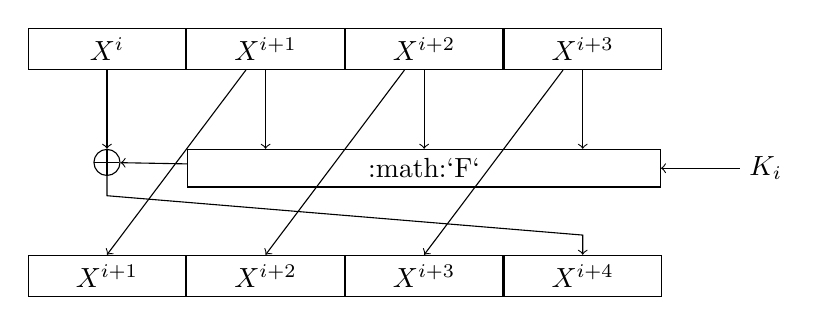
\begin{tikzpicture}
    \node [block] (xi0) {$X^{i}$};
    \node [block, right=0cm of xi0] (xi1) {$X^{i+1}$};
    \node [block, right=0cm of xi1] (xi2) {$X^{i+2}$};
    \node [block, right=0cm of xi2] (xi3) {$X^{i+3}$};

    \node [XOR, below=1cm of xi0] (xor) {};
    \node [below=1cm of xi2, block, minimum width=6cm] (F) {:math:`F`};
    \node [right=1cm of F] (K) {$K_i$};

    \node [block, below=1cm of xor] (xj0) {$X^{i+1}$};
    \node [block, right=0cm of xj0] (xj1) {$X^{i+2}$};
    \node [block, right=0cm of xj1] (xj2) {$X^{i+3}$};
    \node [block, right=0cm of xj2] (xj3) {$X^{i+4}$};

    \draw [->] (xi0) -- (xor);
    \draw [->] (xi1.south) -- (xi1.south |- F.north);
    \draw [->] (xi2.south) -- (xi2.south |- F.north);
    \draw [->] (xi3.south) -- (xi3.south |- F.north);
    \draw [->] (K) -- (F.east);
    \draw [->] (F) -- (xor);

    \draw [->] (xor.south) -- ++(0.0, -0.25) -- ($(xj3.north) + (0.0, 0.25)$) -- (xj3.north);
    \draw [->] ($(xi1.south) + (-0.25, 0)$) -- (xj0.north);
    \draw [->] ($(xi2.south) + (-0.25, 0)$) -- (xj1.north);
    \draw [->] ($(xi3.south) + (-0.25, 0)$) -- (xj2.north);
\end{tikzpicture}
\end{document}